\chapter{Evaluation and Analysis}
The enhancement in the existing software architecture to improve the processing speed of DUT electrical measurements are evaluated and analysed in this chapter. 
The processing capabilities of Reverse Polish Notation and linear scaling function are evaluated by measuring their time and memory consumption in performing the scaling computation. 
In order to compute Reverse Polish Notation or linear scaling function, a piece of code is written in the digital processing module of MicroMoPS. 
Scaling operation is performed as many times as the number of communication channels that are present in the MicroMoPS (see \cref{sec:parse}). The scaling operation comes as a part of the execution of test plans, and the Lua modules or classes that are specific to scaling are used in the test plan script to invoke the corresponding Lua C-API of MoPS-CORE microcontroller firmware. The Lua class that is meant for invoking the scaling function corresponding C-API i.e., `ai\_read\_scaled()' (see \cref{sec:scaling}) is `ai' ~\cite{Steinwender2016}. The real-time performance of the scaling operations is tested by invoking the scaling function multiple times from the TinyHost (see \cref{sec:TinyHost}), while the test plan is not running. Before invoking scaling functions setting some of the configurations (see \cref{fig:tinyhost}) that are specific to the communication channel is necessary. These test runs of a scaling operation are done at a very indeterministic interval to determine the stable values of the time that is consumed by the scaling operation. The time measurements that are recorded during the test runs are approximated to the closest simpler representation.        
The real-time performance of Reverse Polish Notation and linear scaling function is discussed in the following sections. 
%The calculation of time and memory consumption of the "Reverse polish notation" are as follows:

\section*{Real-Time performance of RPN function}

As described in the \cref{sec:scaling}, the `ai\_read\_scaled()' handler makes use of `rpn\_calc()` handler to perform RPN computation. The Memory consumption of the RPN is calculated by investigating the code that is associated in performing the RPN. The code snippet which performs the data processing (RPN) computation is built by using several local variables that are specific to `rpn\_calc()` (see \cref{fig:DP}) handler. The memory consumption of each of the local variables that are part of `rpn\_calc()' is as follows:  
\begin{enumerate}
\item rpn\_string = 32 bytes (max)
\item *temp(char) = 1 byte
\item *delim(char) = 1 byte
\item is valid(bool) = 1 byte
\item *save(char) = 1 byte
\item *snippet(char) = 1 byte
\item lua\_number -- res, a, b (float) = 4bytes*3 = 12 bytes
\end{enumerate}
The sum of the memory consumption of the local variables that are part of `rpn\_calc()' is \textbf{49 bytes}.
\\
\\
Consumption of time in performing RPN function is calculated by making use of the `time\_it()' handler from the `MoPS\_time.c' module. The calculation of the consumption of time is done for around 50 test runs. After around 50 test runs, the range of consumption of time to perform RPN is calculated. The time consumed by the RPN function approximately ranges from \textbf{\SIrange{45}{66}{\micro\second}}.

\section*{Real-Time performance of Linear scaling mechanism}

Similarly, the real-time performance of "Linear scaling mechanism" is measured by calculating the time and memory consumption of the code that performs the computation. 
The Memory consumption of the linear scaling mechanism is calculated by investigating the code that is associated in performing the linear scaling function.
Mere linear scaling equation is implemented within a `ai\_read\_scaled()' handler to perform the processing (linear scaling function) of data. 
The Memory consumption of each of the local variables that are part of linear scaling mechanism is as follows:

\begin{enumerate}
\item scale (float) = 4 bytes
\item digital\_result (float) = 4 bytes
\item offset (float) = 4 bytes 
\end{enumerate}                         
The sum of the memory consumption of the local variables that are part of linear scaling function is \textbf{12 bytes}.

The method of calculation of time consumption remains the same as how it is done for RPN function. Also, for the calculation of consumption of time to compute linear scaling function, around 50 samples of measurements are taken. The time consumed by linear scaling mechanism approximately ranges from \textbf{\SIrange{29}{134}{\nano\second}}.

\begin{figure}[hbt]
		\centering
		%\makebox[\textwidth]{%
		%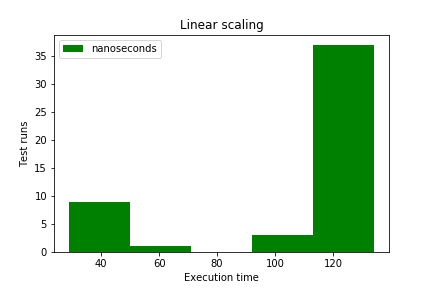
\includegraphics[trim=0 55 0 210, clip, width=210mm, scale=0.75]{images/linear_scaling.png}
		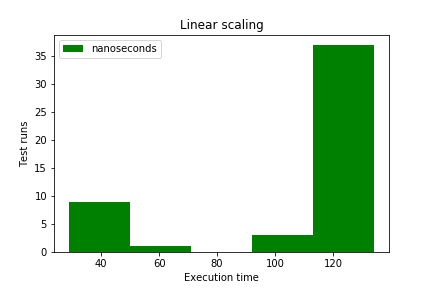
\includegraphics[width=0.6\textwidth]{images/linear_scaling.png}
		%\hfill
		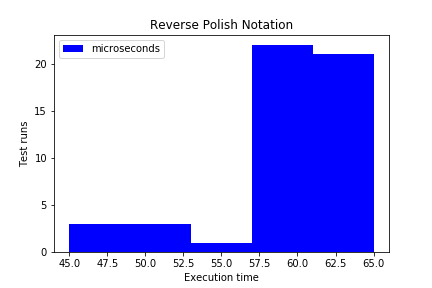
\includegraphics[width=0.6\textwidth]{images/rpn.png}
		\caption{Distribution of execution time of the scaling functions}
		\label{fig:Histogram}
\end{figure}

The distribution of the execution time of the linear scaling and Reverse Polish Notation function is as shown in the \cref{fig:Histogram}. The test runs of scaling computation are performed in this sophisticated stress test environment to record the time that is consumed by the scaling operation. At rare times the execution time of the scaling computation lies closer towards the \gls{BCET} of the given scaling computation because of the less interrupt load during the scaling operation. However, most of the other times the execution time of the scaling computation varies around the \gls{WCET} of the given scaling computation because of the substantial interrupt load during the scaling operation. In the case of a linear scaling mechanism, out of 50 disordered test runs, 8 to 10 test runs that records the execution time lies between 29 and 70 nanoseconds, and the rest of the test runs that records the execution time lies between 95 and 134 nanoseconds. Similarly, in the case of Reverse Polish Notation, out of 50 disordered test runs, 2 to 4 test runs that records the execution time lies between 45 and 57.5 microseconds, and the rest of the test runs that records the execution time lies between 57.5 and 65 microseconds. From the obtained execution time distribution, it can be inferred that there exists the stable region around the \acrshort{WCET}, which means almost all the times regardless of the increase or decrease of test runs from 50, the execution time of scaling operation only keeps moving within the stable region and at rare times towards the \acrshort{BCET}. 
The stable region for Reverse Polish Notation and linear scaling function lies between 95 and 134 nanoseconds, and 57.5 and 65 microseconds, respectively.            

The real-time performance comparison of Reverse Polish Notation and linear scaling mechanism is as shown in the Table 6.1.

\begin{table}[hpt]
	\centering
	\label{Table:scaling}
	\caption{Real-time performance comparision}
	\begin{tabular}{|p{4cm}||p{2.5cm}|p{2.7cm}||p{2.7cm}| } 
 	\hline
 	\textbf{Scaling mechanism}   &\textbf{Time}    &\textbf{Memory}    &\textbf{Test runs}\\
 							&\textbf{consumption}    &\textbf{consumption}  &\textbf{}\\
 	\hline
	RPN   &{45 $\mu$s - 66 $\mu$s}   &49 bytes &{$\approx$50}\\
 	\hline
	Linear scaling   &{29 ns - 134 ns}   &12 bytes &{$\approx$50}\\
 	\hline
	\end{tabular}
\end{table}

%\begin{figure}[hbt]
%		\centering
	%	%\makebox[\textwidth]{%
		%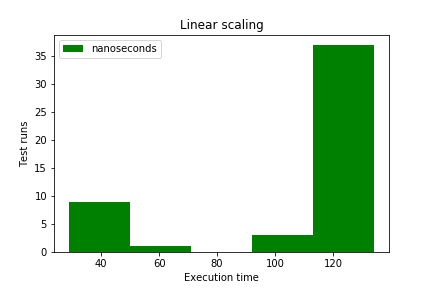
\includegraphics[trim=0 55 0 210, clip, width=210mm, scale=0.75]{images/linear_scaling.png}
		%\begin{minipage}[b]{0.9\textwidth}
		%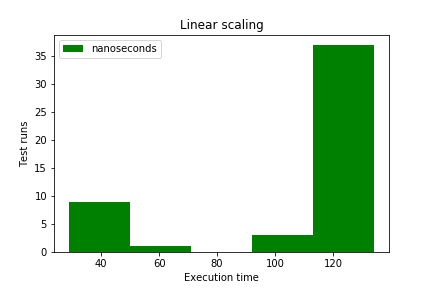
\includegraphics[width=0.4\textwidth]{images/linear_scaling.png}
		%\hfill
		%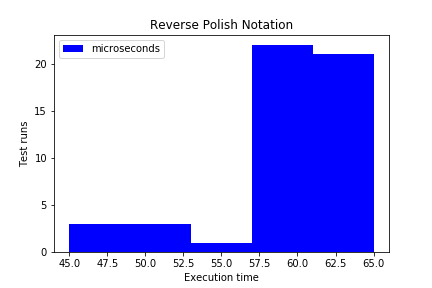
\includegraphics[width=0.5\textwidth]{images/rpn.png}
		%\caption{Distribution}
		%\label{fig:Histogram}
		%\end{minipage}
		%\hfill
		%\begin{minipage}[b]{0.9\textwidth}
		%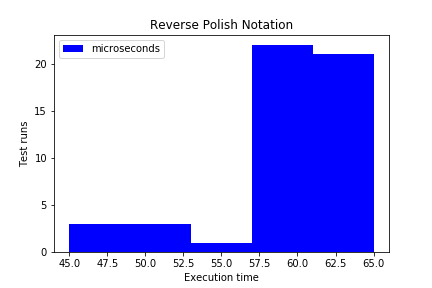
\includegraphics[width=0.4\textwidth]{images/rpn.png}
		%\hfill
		%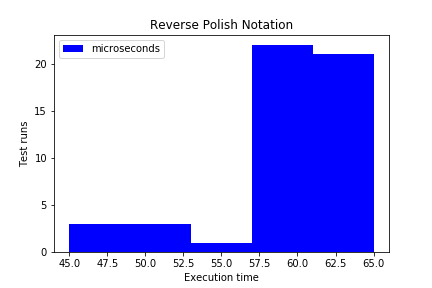
\includegraphics[width=0.5\textwidth]{images/rpn.png}
		%\caption{Distribution}
		%\label{fig:Histogram2}
		%\end{minipage}
%\end{figure}


%\begin{figure}[hbt]
	%	\centering
		%\makebox[\textwidth]{%
		%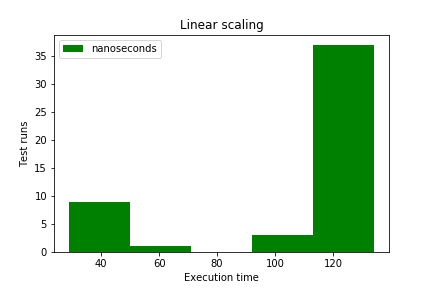
\includegraphics[trim=0 55 0 210, clip, width=210mm, scale=0.75]{images/linear_scaling.png}
		%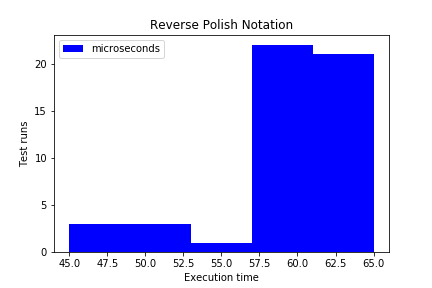
\includegraphics[width=0.5\textwidth]{images/rpn.png}
		%%\hfill
		%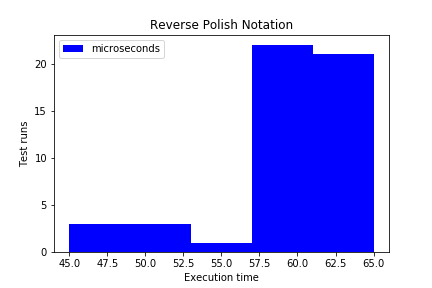
\includegraphics[width=0.5\textwidth]{images/rpn.png}
		%\caption{Distribution of execution time of the scaling functions}
		%\label{fig:Histogram2}
%\end{figure}

From Table 6.1, it can be concluded that the linear scaling mechanism consumes less time and memory in comparison with the Reverse Polish Notation function. 
This, further implies that the linear scaling mechanism is more real-time efficient scaling mechanism compared to Reverse Polish Notation. 

On the other hand, the entire procedure of resolution of board UIDs from multiple different sources such as the test plan, board and scaling database in web server, board UIDs communication from MicroMoPS, and subsequent communication of scaling parameters to the data processing system of MicroMoPS supports to an automation of processing of analog measurements in the stress test environment regardless of any plausible combination of hardware target, application module and DUT.
Every plausible combination of boards correspond to an individual type of stress test application. The main benefit of the automation of the processing of data is the avoidance in the maintenance of the scaling database of every application-specific stress test system in the control module. This results in a conservation of quite an amount of memory of the MicroMoPS. Also, by automating the processing of data, the method of manual feed of scaling values is avoided, which helps in minimizing human error.  
%As a result, the scaling operation is automatically performed irrespective of the stress test applications that are performed. 

\section{Answers to the Research questions}
The above analysis and evaluation of the results bring a conclusion to the raised research questions (see \cref{sec:RQs}).

\begin{itemize}
	\item By analysis of the various existing application boards, a linear model solution could be found.
		The performance of the linear model over the Reverse Polish Notation model is greatly enhanced. 
	\item The derivation of a linear scaling mechanism and their precise conversion of analog measurements into control module-specific voltages, proves the possibility of a linear scaling mechanism in this stress test environment. 
	\item The resolution of board UIDs and the filtering of scaling values establishes the automation of data processing.
		This exhibits the possibility of automated processing of analog measurements in this stress test environment.  
\end{itemize}
%\begin{tabular}{ |p{3cm}|p{5cm}|p{2cm}| }
 %\hline
 %\multicolumn{3}{|c|}{Real-time performance comparision } \\
 %\hline
 %\textbf{Scaling mechanism}   & \textbf{Time consumption}    &\textbf{Memory consumption} \\
%RPN   &45 us - &66 us   &49 bytes \\
%Linear scaling   &29 ns - 134ns   &12 bytes \\
 %\hline
%\end{tabular}
%\label{Table5}
